\chapter{Vision-Language Prompting for Panoptic Scene Graph Generation}

\begin{tcolorbox}[
    breakable,
    colback=gray!5,
    colframe=black,
]
The content of this chapter corresponds to the paper: \\
\noindent \textbf{VLPrompt-PSG: Vision-Language Prompting for Panoptic Scene Graph Generation} \\
\noindent Zijian Zhou, Holger Caesar, Qijun Chen, Miaojing Shi \\
\noindent \textit{International Journal of Computer Vision (IJCV), 2025}.

\vspace{0.6em}
\noindent \textbf{Statement of individual contribution.}
This work was carried out within my doctoral research at King's College London. I identified the research problem, developed the method, implemented the models, designed and ran all experiments, performed the analysis, and wrote the manuscript. My co-authors contributed supervisory guidance on research direction, formulation, experimental design, and writing. Section~\ref{sec:individual_contributions} gives the corresponding statement for every chapter of this thesis.
\end{tcolorbox}

\section{Motivation}
Building on the long-tail modeling of Chapter~3, this chapter studies a second limitation of closed-set PSG: many rare or ambiguous relations cannot be resolved reliably from visual evidence alone.
Prior methods mainly rely on vision features or only use minimal language cues such as category names, leaving rich relational commonsense largely unused.
Leveraging recent progress in large language models (LLMs), this chapter introduces the \textbf{V}ision-\textbf{L}anguage \textbf{Prompt}ing (\textbf{VLPrompt}) model, which combines object-pair visual features with context-rich language descriptions generated by LLMs.
Through an attention-based prompter network, VLPrompt uses language as a grounded auxiliary signal for relation prediction, particularly for rare predicates.
Experiments on the PSG dataset show that this language-assisted formulation substantially improves performance over previous closed-set PSG methods.
Within the thesis, this chapter is the second step of the PSG line, before Chapter~5 extends the problem to open-set relation prediction.

\section{Introduction}
\label{vlprompt:sec:introduction}

Building on Chapter~3, this chapter addresses a second obstacle to learning relational structure: rare and ambiguous relations are often difficult to resolve from visual evidence alone.
The setting remains closed-set PSG, but the model now incorporates language-derived relational knowledge. Under the argument in Section~\ref{sec:unifying_argument}, access to this knowledge is insufficient unless it is aligned with the relevant object pair and grounded in visual evidence. This chapter therefore learns when and how language features should inform relation prediction.

Panoptic scene graph generation (PSG)~\citep{yang2022panoptic} extends scene graph generation (SGG)~\citep{lu2016visual} by incorporating panoptic segmentation~\citep{kirillov2019panoptic} to capture richer and more detailed representations of images, including both ``thing''~\citep{lin2014microsoft} and ``stuff''~\citep{caesar2018coco} object classes.
PSG constructs a directed graph to represent an image, where nodes signify objects and edges capture the relations between objects.
As a bridge between vision and language~\citep{zhu2022scene}, PSG has a multitude of downstream applications such as visual question answering~\citep{hildebrandt2020scene}, image captioning~\citep{gao2018image, chen2020say}, and visual reasoning~\citep{aditya2018image, shi2019explainable}; furthermore, it can also benefit relevant fields like embodied navigation~\citep{singh2023scene} and robotic action planning~\citep{amiri2022reasoning}.

Notwithstanding, the current performance of PSG~\citep{yang2022panoptic, zhou2023hilo, wang2023pair, li2023panoptic, hayder2024dsgg, lorenz2024fair, zhou2025openpsg} remains unsatisfactory, limiting its downstream applications.
The essential reason lies in the severe long-tail problem in relation categories: for instance, in the PSG dataset~\citep{yang2022panoptic}, the top three most frequent relation categories account for over 50\% of entire samples, with numerous rare relations appearing less than 1\%.
PSG models thus struggle to accurately predict these rare relations.

Recent methods~\citep{lyu2022fine, dong2022stacked, li2022ppdl, zhang2022fine, deng2022hierarchical, zhou2023hilo, yu2023visually, hayder2024dsgg, im2024egtr, li2024leveraging, lorenz2024fair} have made progress in addressing the long-tail problem, mainly exploiting the strength of vision information for relation prediction, whilst overlooking the language information in PSG.
The integration of language information is however important to provide additional common sense knowledge for objects and their relations. 
For example, in the two images of Fig.~\ref{vlprompt:fig:motivation}, the relation between the person and the elephant is \textit{cleaning}.
In the image 2 of Fig.~\ref{vlprompt:fig:motivation}, where the person is on the elephant's back \textit{cleaning} it, this scenario can easily lead previous vision-only models to classify the relation as \textit{riding}.
In contrast, our vision-language model can utilize language information like ``a person cleans an elephant using brushes on the back of the elephant'', thus precisely predicting the relation as \textit{cleaning}.

In SGG task, some methods~\citep{he2022towards, dong2022stacked} have recognized the importance of incorporating language information besides vision. 
However, the way language information is utilized in these works is limited to category names of objects or relations, providing no further context and hence not fully addressing the long-tail problem.
The same observation goes to methods like~\citet{gu2019scene, zareian2020bridging}, which integrate knowledge graphs into the SGG task.
With the rapid development of Large Language Models (LLMs)~\citep{chatgpt, touvron2023llama}, acquiring richer language information, instead of merely the concepts of objects or relations, becomes much easier than before.

\begin{figure}[t]
    \centering
    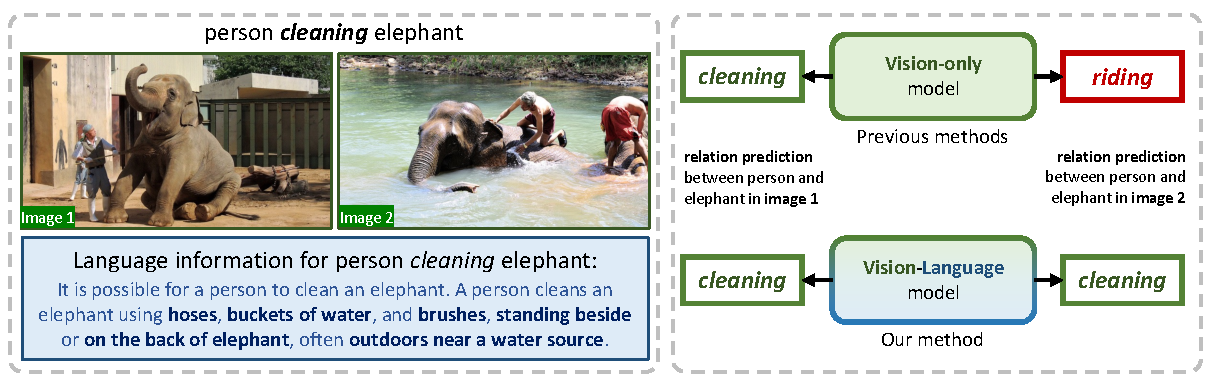
\includegraphics[width=1.0\linewidth]{Chapter4/Figures/motivation_v4.pdf}
    \caption{Comparison between previous PSG methods and ours.
    \textbf{Left}: Images of ``person \textit{cleaning} elephant'' in two different scenes, accompanied by snippets of descriptions about ``person \textit{cleaning} elephant'' obtained from LLMs.
    \textbf{Right}: Previous vision-only models can predict the \textit{cleaning} relation between the person and elephant in image 1, but often classify image 2's relation as \textit{riding} due to the person's position on the back of the elephant.
    Our vision-language model, enriched with language information, precisely identifies the \textit{cleaning} relation in both images.
    }
    \label{vlprompt:fig:motivation}
\end{figure}

This chapter introduces a novel \textbf{V}ision-\textbf{L}anguage \textbf{Prompt}ing (\textbf{VLPrompt}) model, which leverages rich language information from LLMs to help predict relations between objects in visual images.
The language information serves as a powerful supplement to relation prediction, especially for rare ones.
Our model comprises three parts, forming a complete system implementation of our proposed idea.
The first is the \emph{vision feature extractor}, where we process the input image with a panoptic segmentation network adapted from Mask2Former~\citep{cheng2022masked} to extract features of different objects.
We pair and concatenate these object features and integrate their corresponding spatial information to form the vision prompting features.
In contrast, in the second part, the \emph{language feature extractor}, we employ the chain-of-thought technique~\citep{wei2022chain} to design various prompts, aiming to stimulate LLMs to propose context-rich language information for potential relations between a subject-object pair or judge a specific subject-relation-object triplet.
These two functions are realized via the carefully designed relation proposer prompt and relation judger prompt.  
Subsequently, these language descriptions are transformed into language features using a pre-trained text encoder.
Finally, in the third part, the \emph{vision-language prompter}, we design a novel dual attention-based prompter network to facilitate the interaction between vision features and the two complimentary language features respectively, resulting into two sets of relation predictions.
They are combined via a MLP-based gating network to take the strength of both for final relation prediction.
The whole VLPrompt is trained end-to-end.

Extensive experiments on the PSG dataset~\citep{yang2022panoptic} demonstrate that our VLPrompt significantly enhances the PSG performance, especially in predicting rare relations, highlighting the importance of integrating language information from LLMs to support relation prediction in the PSG task.
Within the thesis, VLPrompt forms the second step of the PSG progression: Chapter~3 established a stronger visual baseline for long-tail relation prediction, this chapter adds language-assisted reasoning on top of that closed-set setting, and Chapter~5 then extends the same line to open-set PSG.

\section{Related Work}
\label{vlprompt:sec:related_work}

\subsection{Scene Graph Generation}
\label{vlprompt:sec:sgg}

Scene graph generation (SGG)~\citep{lu2016visual} is a crucial task in scene understanding and has garnered widespread attention in the computer vision community.
In recent years, numerous methods~\citep{xu2017scene, zellers2018neural, tang2019learning, lin2020gps, li2022sgtr, shit2022relationformer, zhang2022fine, yu2023visually, hayder2024dsgg, im2024egtr, li2024leveraging, li2025fine} have achieved notable progress.
Various model architectures have been proposed, such as intricately designed message passing structures~\citep{li2017vip, dai2017detecting, li2017scene, zellers2018neural, gu2019scene, hu2022neural}, attention-based networks~\citep{zheng2019visual, qi2019attentive}, tree-based networks~\citep{zhang2017visual, hung2020contextual}, DETR-based networks~\citep{li2022sgtr, shit2022relationformer, cong2023reltr} and transformer-based networks~\citep{hayder2024dsgg, im2024egtr}.
Specifically, to address the long-tail problem, some methods enhance the prediction accuracy of rare relations through data re-sampling~\citep{li2021bipartite} and loss re-weighting~\citep{kang2023skew}.
Relevant techniques that have been developed include constructing enhanced datasets~\citep{zhang2022fine, yu2023visually}, grouping relations for training~\citep{dong2022stacked}, constructing multi-stage hierarchical training~\citep{deng2022hierarchical}, and designing de-bias loss functions~\citep{yu2020cogtree, kang2023skew}.
Most methods leverage images as sole inputs.
Besides, some methods~\citep{lu2016visual, hwang2018tensorize, liao2019natural, zhang2019large, dupty2020visual, zhong2021learning, ye2021linguistic} have begun exploring language information or knowledge graphs in SGG; specifically, the explored language information is so far confined to basic language concepts of objects or relations.


\subsection{Panoptic Scene Graph Generation}
\label{vlprompt:sec:psg}

Panoptic scene graph generation (PSG)~\citep{yang2022panoptic} has emerged as a novel task in scene understanding in recent years.
Unlike SGG~\citep{lu2016visual}, PSG employs panoptic segmentation~\citep{kirillov2019panoptic} instead of bounding boxes to represent objects, enabling a more comprehensive understanding.
Similar to SGG methods, current methods in PSG~\citep{yang2022panoptic, zhou2023hilo, wang2023pair, li2023panoptic, hayder2024dsgg, lorenz2024fair} also mainly rely on the image input and do not utilize any language information.
For instance, PSGTR~\citep{yang2022panoptic} build a baseline PSG model by adding a relation prediction head to DETR~\citep{carion2020end}.
PSGFormer~\citep{yang2022panoptic} advances PSGTR by separately modeling objects and relations in two transformer decoders and introducing an interaction mechanism. 
Recently, HiLo~\citep{zhou2023hilo} addresses the long-tail problem by specializing different network branches in learning both high and low frequency relations. 
PairNet~\citep{wang2023pair} develops a novel framework using a pair proposal network to filter sparse pairwise relations, improving PSG performance.
TextPSG~\citep{zhao2023textpsg} leverages language information for model training but adopts a semi-supervised approach without applying language information to a fully supervised method, resulting in poor performance.
DSGG~\citep{hayder2024dsgg} builds a transformer-based network with graph-aware queries to predict unbiased relations.
In addition, some works~\citep{yang2023panoptic, yang20234d} extend panoptic scene graph generation to video~\citep{yang2023panoptic} and 4D~\citep{yang20234d} scenes.
In contrast to previous methods that rely solely on vision as input, we propose a fully supervised PSG method that leverages both vision and language inputs.


\subsection{Large Language Models for Vision Tasks}
\label{vlprompt:sec:llm}
LLMs have led to large improvements in natural language processing tasks~\citep{min2023recent}.
They are normally trained on extensive text corpora by learning to autoregressively predict the next word, hence encapsulate a broad spectrum of common sense knowledge of linguistic patterns, cultural norms, and basic worldly facts.
Prominent examples of LLMs include GPT series~\citep{chatgpt}, Llama series~\citep{touvron2023llama1, touvron2023llama}, Gemini~\citep{gemini}, and Claude~\citep{claude}, with Llama series being open-source publicly available.
Given the extensive common sense information contained in LLMs, some researchers start to propose multimodal sockets to LLMs~\citep{zhang2024vision, wu2024towards} and apply them to various vision tasks, such as recognition~\citep{huang2023inject, wang2023all}, detection~\citep{tang2023cotdet, zhang2023next, qi2024generalizable}, segmentation~\citep{lai2023lisa, zhou2023text, xia2024gsva}, visual question answering~\citep{liu2023large, xenos2023simple}, image reasoning~\citep{chen2023large, zhang2024omg} and robotic navigation~\citep{tsai2023multimodal, shah2023lm}; nevertheless, there are no such models specifically designed for panoptic scene graph generation so far.
In contrast, our method designs various prompts to stimulate LLMs to elicit rich language information to enhance relation prediction.

\section{Method}
\label{vlprompt:sec:method}

In this section, we introduce our method, \textbf{VLPrompt}.
Given an image $\mathcal{I} \in \mathbb{R}^{H \times W \times 3}$ and language description $\mathcal{T}$ generated from LLMs, we extract vision and language features from them to predict panoptic scene graph $\mathcal{G} = \{\mathcal{O}, \mathcal{R}\}$, \ie, $\mathcal{G} = \text{VLPrompt} (\mathcal{I}, \mathcal{T})$.
In $\mathcal{G}$:
\begin{itemize}
    \item $\mathcal{O} = \{o_i\}_{i=1}^{N}$ signifies $N$ objects segmented from the image $\mathcal{I}$.
    Each object is defined by $o_i = \{c, m\}$, where $c$ belongs to one of the predefined $C$ object categories, and $m$ is a binary mask in $\{0, 1\}^{H \times W}$ for this object.
    \item $\mathcal{R} = \{r_{i,j} \mid i,j \in \{1, 2, \ldots, N\}, i \neq j\}$ denotes relations with $r_{i,j}$ being the relation between $o_i$ and $o_j$. Each $r$ belongs to one of the predefined $K$ relation categories (or no relation), $N$ is the number of objects in the image. 
\end{itemize}

\begin{figure}[t]
    \centering
    % \fbox{\rule{0pt}{2in} \rule{1.0\linewidth}{0pt}}
    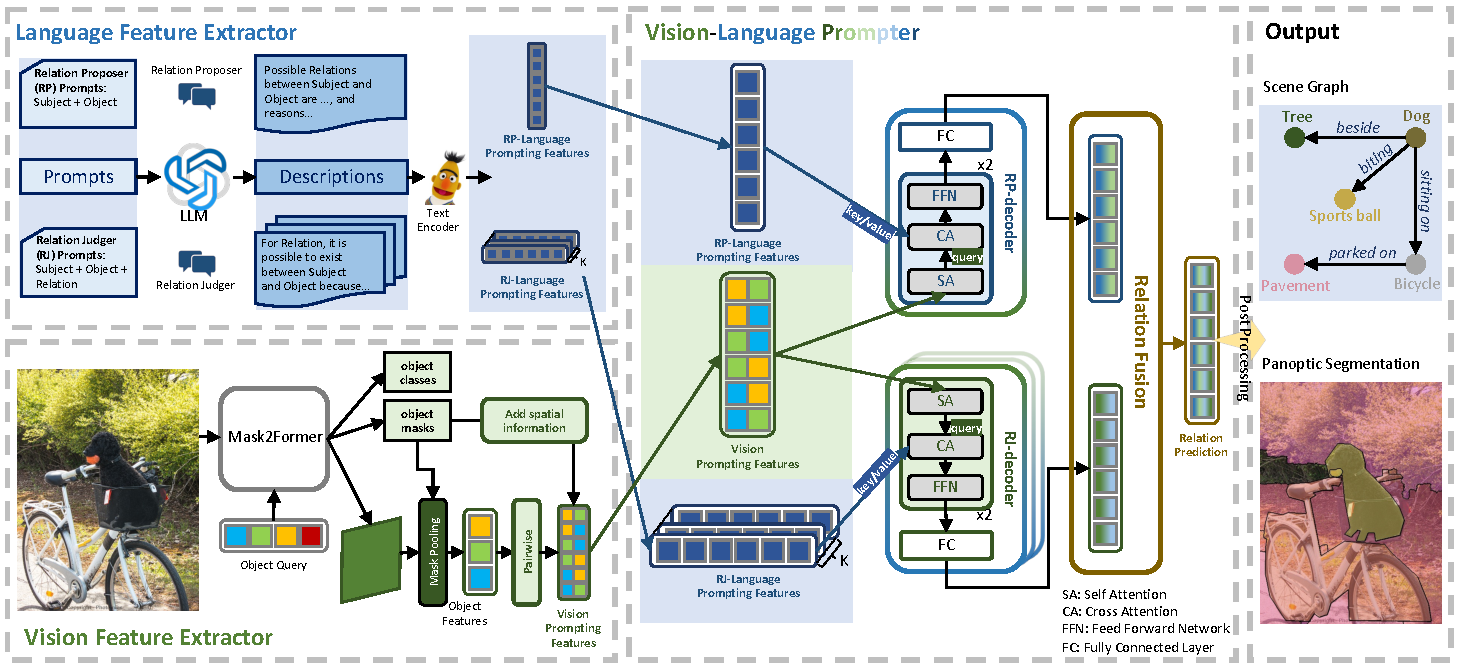
\includegraphics[width=1.0\linewidth]{Chapter4/Figures/overview_v3.pdf}
    \vspace{-4mm}
    \caption{The overall framework of VLPrompt, which comprises three components: the vision feature extractor, the language feature extractor and the vision-language prompter.
    We employ the language feature extractor to obtain LLM-based language information and integrate it into the final relation prediction through the vision-language prompter, enabling unbiased relation predictions.}
    \label{vlprompt:fig:overview}
\end{figure}

As shown in Fig.~\ref{vlprompt:fig:overview}, our method comprises three main components: \textit{vision feature extractor}, \textit{language feature extractor}, and \textit{vision-language prompter}.
The \textit{vision feature extractor} (Sec.~\ref{vlprompt:sec:vision_feature_extractor}) adapts from a segmentation network (\eg, Mask2Former~\citep{cheng2022masked}) to predict object masks and form subject-object pairs for feature extraction, which result into vision prompting features.
For the \textit{language feature extractor} (Sec.~\ref{vlprompt:sec:language_feature_extractor}), we generate different types of descriptions by leveraging the extensive common sense knowledge embedded in LLMs through carefully designed prompts, which is beneficial for relations of different frequencies.
These descriptions are then converted into language prompting features using a text encoder.
Next, the vision and language prompting features are fed into a \textit{vision-language prompter} (Sec.~\ref{vlprompt:sec:vision_language_prompter}), where vision prompting features interact with different types of language prompting features respectively, so as to take advantage of the complimentary language information to assist relation predictions. 
Finally, these relation predictions are combined by a relation fusion module to achieve the final relation prediction.


\subsection{Vision Feature Extractor}
\label{vlprompt:sec:vision_feature_extractor}

Given an image $\mathcal{I}$, we first leverage Mask2Former~\citep{cheng2022masked} to produce $N$ objects with masks.
They are formed into $N \times (N-1)$ subject-object pairs by pairing any two distinct ones. 
The purpose of the vision feature extractor is to extract vision prompting feature for each subject-object pair, which includes visual features from the segmentation network itself as well as spatial features between the subject-object pairs.
In this way, we can enhance the representations of the relations between subject-object pairs.  

\noindent \textbf{Subject-object visual features.}
We first obtain the features corresponding to each object.
Considering that the output feature map by the pixel decoder in Mask2Former retains rich information of the image, we use mask pooling to obtain object features corresponding to the $N$ objects from the feature map based on each object's mask $m$.
Then, we pair and concatenate any two distinct object features to form $N \times (N-1)$ subject-object visual features $F_{V}^{vi}$.

\noindent \textbf{Subject-object spatial features.}
To further enhance the representations of subject-object pairs, especially their spatial relations,  we are inspired by~\citet{peyre2017weakly} to encode the spatial features into the subject-object visual features.
Specifically, given $o_i$ and $o_j$ corresponding to subject and object, we first derive their encompassing bounding boxes $b_i=[x_i, y_i, w_i, h_i]$ and $b_j=[x_j, y_j, w_j, h_j]$, where $(x, y)$ is the center of the bounding box, and $(w, h)$ are the width and height.
Next we construct spatial features: 
\begin{equation}
    v(o_i, o_j) = [\frac{x_{j} - x_{i}}{\sqrt{w_{i}h_{i}}}, \frac{y_{j} - y_{i}}{\sqrt{w_{i}h_{i}}}, \sqrt{\frac{w_{j}h_{j}}{w_{i}h_{i}}}, \frac{b_i \cap b_j}{b_i \cup b_j}, \frac{w_i}{h_i}, \frac{w_j}{h_j}],
\end{equation}
where $v(o_i, o_j)$ encodes the spatial relation between $o_i$ and $o_j$, such as the ratio of their bounding box sizes, the overlap between two objects and the aspect ratio of each object.
Then, we use a FC layer to expand the spatial features to the same dimension as $F_{V}^{vi}$, resulting in $F_{V}^{sp}$.

Finally, we apply a FC layer to the sum of $F_{V}^{vi}$ and $F_{V}^{sp}$ and output vision prompting features $F_V \in \mathbb{R}^{N \times (N-1) \times D_{V}}$, where $D_{V}$ is the vision feature dimension.


\subsection{Language Feature Extractor}
\label{vlprompt:sec:language_feature_extractor}

The purpose of the language feature extractor is to leverage the extensive common sense knowledge embedded in LLMs for providing additional language information to the PSG task, which can mitigate the long-tail problem in relation prediction.
To achieve this, we need to design various prompts to elicit outputs from LLMs.
On one hand, LLMs can act as a relation proposer, suggesting possible relations between two objects, which often are frequently occurring relations in the real world.
On the other hand, LLMs can also serve as a relation judger, given a subject-object pair and their specific relation, LLMs make judgment and provide reasoning for this relation. This allows detailed descriptions even for rare relations.
Specifically, we design two types of prompts: relation proposer prompt (RP-Prompt) for proposing and explaining potential relations given a subject-object pair; relation judger prompt (RJ-Prompt) for judging and reasoning  upon a specific subject-relation-object triplet. 
Below, we detail how to obtain RP- and RJ-language prompting features based on the generated descriptions.

\noindent \textbf{RP-language prompting feature.}
For RP-language prompting feature, we stimulate LLMs to guess all possible relations between two given objects $o_i$ and $o_j$, along with explanation for these relations.
To achieve this, we utilize the chain-of-thought technique~\citep{wei2022chain}: we engage in a dialogue with an LLM (\eg, GPT-4~\citep{chatgpt}), initially informing it to act as a relation proposer and defining the task.
Then an example is provided to the LLM to clarify its role.
We explicitly mention the predefined $K$ relations in the prompt, guiding the LLM to propose from them.
Finally, a certain subject-object pair ($o_i$ and $o_j$) is given to the relation proposer prompt.
By giving this prompt to the LLM, we obtain the description for potential relations between $o_i$ and $o_j$.
For predefined relations that are not proposed by the LLM, we would append a template phrase by the end of the description, such as ``It is not likely for $o_i$ and $o_j$ to have relation $r$.'', to ensure that the language description clearly distinguishes common from uncommon relations and comprehensively covers all relation categories.
To encode the description into a feature interpretable by our model, we use a text encoder (\eg, OpenAI Embeddings~\citep{chatgpt}) to convert the description into the feature $F_{L(i, j)}^{RP} \in \mathbb{R}^{1 \times D_{L}}$, namely RP-language prompting feature.
This process consolidates all descriptions (each expressing multiple plausible relations for a given subject-object pair) into a single feature, allowing for a condensed reflection of the distinct attributes of common relations between subject and object.

\noindent \textbf{RJ-language prompting feature.}
For RJ-language prompting feature, we design the relation judger prompt: 
we not only provide two objects $o_i$, $o_j$ but also specify a relation $r_{k}$ between them. 
By using the common sense knowledge, the LLM judges whether the relation $r_{k}$ could plausibly exist between $o_i$ and $o_j$ and provides reason.
Similar to above, we use the chain-of-thought technique~\citep{wei2022chain} by telling the LLM that it serves as a relation judger; we first define the task, then give the example, and finally, the triplet ($o_i\text{-}r_{k}\text{-}o_j$) is provided.
Following the same process as for RP-language prompting feature, we feed the relation judger prompt to the LLM to obtain the language description and leverage the text encoder (same as above) to encode it into the RJ-language prompting feature $F_{L(i, j, k)}^{RJ} \in \mathbb{R}^{1 \times D_{L}}$. Different from the RP-language prompting feature, we encode each relation triplet into an individual feature, storing more detailed and subtle information for each relation, hence favouring rare relations.

By enumerating all $C$ objects and $K$ relations in the dataset, we derive all RP- and RJ-language prompting features.
To further enhance the practicality of our method and avoid repeatedly invoking LLM at runtime, we store them in a database.
Given an image with $N$ objects, we retrieve two sets of features, $F_{L}^{RP} \in \mathbb{R}^{N \times (N-1) \times D_{L}}$ and $F_{L}^{RJ} \in \mathbb{R}^{N \times (N-1) \times K \times D_{L}}$ from the database.
Note that for a specific relation $r_{k}$ between all subject object pairs in this image, the RJ-language prompting feature is denoted as $F_{L(k)}^{RJ} \in \mathbb{R}^{N \times (N-1) \times D_{L}}$.


\subsection{Vision-Language Prompter}
\label{vlprompt:sec:vision_language_prompter}

To enable the vision prompting feature to predict relations from both macro and detailed perspectives, we let $F_V$ interact with $F_L^{RP}$ and $F_L^{RJ}$ through two separate decoders, termed as RP-decoder and RJ-decoder, responsible for the interaction from $F_V$ to $F_L^{RP}$ and $F_L^{RJ}$, respectively. 
Each decoder contains two standard transformer decoder blocks~\citep{vaswani2017attention}, followed by a FC layer for relation prediction.
The predictions from the two decoders are complementary: the RP-language prompting feature focuses on the condensed and distinct attributes of frequently occurring relations for a given subject-object pair; in contrast, the RJ-language prompting feature focuses on the detailed and subtle attributes of every possible relation (common or rare) for the subject-object pair. A relation fusion module consisting of a gating network is thereby devised by the end to fuse the relation predictions from both decoders into the final one. Before feeding $F_V$, $F_L^{RP}$, and $F_L^{RJ}$ into different decoders, we use a FC layer to transform their dimensions to a uniform dimension $D$. Below, we specify the RP-decoder, RJ-decoder, and the relation fusion module, respectively.

\noindent \textbf{RP-decoder.}
The RP-decoder aims to utilize the $F_{L}^{RP}$ to assist $F_{V}$ in relation prediction, particularly for relations that are frequently encountered between $o_i$ and $o_j$ in the real world.
In the first transformer decoder block, $F_{V}$ is firstly fed into the self-attention layer, primarily aggregating the visual relational information in $F_{V}$.
Afterwards, the self-attended $F_{V}$ as query and the $F_{L}^{RP}$ as key/value are engaged in the subsequent cross-attention layer,
 aggregating the common sense knowledge of potential relations between $o_i$ and $o_j$ into $F_{V}$. 
The output is further processed through a feed-forward network.
In the second transformer decoder block, we repeat the aforementioned process.
Finally, a fully connected layer is used to transform feature dimension $D$ to the number of relations $K$, and a sigmoid function is applied afterwards to obtain $R^{RP} \in \mathbb{R}^{N \times (N-1) \times K}$. 

\noindent \textbf{RJ-decoder.}
The RJ-decoder aims to facilitate interaction between the RJ-language prompting feature $F_{L}^{RJ}$ with the vision prompting feature $F_{V}$.
Since $F_{L}^{RJ}$ a group of individual language prompting feature for every relation triplet ($o_i\text{-}r_{k}\text{-}o_j$), $F_V$ thus has the opportunity to interact with each relation's language representation independently, which can be particularly beneficial to rare relations.
We conduct parallel interactions between $F_V$ and the $K$ triplet features contained in $F_L^{RJ}$.
For each triplet, the interaction process between $F_V$ and $F_{L(k)}^{RJ}$ is the same to that of the RP-decoder, except that the final FC layer is now only responsible for predicting the probability of certain relation between $o_i$ and $o_j$. The FC layer is used to transform the feature dimension from $D$ to 1.
Finally, we concatenate the respective outputs to get the predictions for all $K$ relations, a sigmoid function is applied over them to obtain $R^{RJ} \in \mathbb{R}^{N \times (N-1) \times K}$.

\noindent \textbf{Relation Fusion.}
Upon obtaining $R^{RP}$ and $R^{RJ}$, we aim to take the strength of both via a relation fusion module.
We devise a gating network consisting of 3-layer MLP to generate two sets of weights, $W^{RP}$ and $W^{RJ}$, each matching the shape of $R^{RP}$ and $R^{RJ}$.
We use the sum of $F_V$ and $F_{L}^{RP}$ as the input of the gating network, and output $W^{RP}$.
For $W^{RJ}$, we use the sum of $F_V$ and the mean of $F_{L}^{RJ}$ along the relation dimension as input to the gating network.
$W^{RP}$ and $W^{RJ}$ are used to element-wisely multiply with $R^{RP}$ and $R^{RJ}$ respectively and the final relation prediction $R$ is a weighted combination:
\begin{equation}
    R = W^{RP} \odot R^{RP} + W^{RJ} \odot R^{RJ},
\end{equation}
where $\odot$ is element-wise multiplication, and $R \in \mathbb{R}^{N \times (N-1) \times K}$.

Finally, the prediction $R$, combined with the object categories and masks predicted by the vision feature extractor, forms the panoptic scene graph $\mathcal{G}$.


\subsection{Model Training}
\label{vlprompt:sec:model_training}
Our model training comprises two parts.
The first part is the segmentation loss $\mathcal{L}_{seg}$ used in the vision feature extractor for panoptic segmentation, we simply follow the loss used in~\citet{cheng2022masked}.
The second part is the relation loss. Since the same subject-object pair might have multiple relations, we use a binary cross-entropy loss~\citep{su2022zlpr}.
To effectively train the vision-language prompter, we apply the relation loss separately to $R^{RP}$, $R^{RJ}$, and $R$ and sum them up as the final relation loss, denoted by  $\mathcal{L}_{rel}$.
The final loss $\mathcal{L}$ is
\begin{equation}
    \mathcal{L} = \lambda \mathcal{L}_{seg} + \mathcal{L}_{rel},
\end{equation}
where $\lambda$ is the weighting coefficient.
In the language feature extractor, we directly utilize pre-trained LLMs, thus eliminating the need for additional model training.

\section{Experiments}
\label{vlprompt:sec:experiments}


\subsection{Datasets}

\textbf{Panoptic Scene Graph (PSG) dataset}~\citep{yang2022panoptic}.
This is the first dataset dedicated to the PSG task, comprising 48,749 annotated images, including 2,186 test images and 46,563 training images.
The dataset includes 80 ``thing''~\citep{lin2014microsoft} and 53 ``stuff'' categories~\citep{caesar2018coco}, as well as 56 relation categories.

\noindent \textbf{Visual Genome (VG) dataset}~\citep{krishna2017visual}.
This dataset is widely used in the SGG task.
To validate our method, we also conduct experiments on the VG dataset.
Following previous works~\citep{zellers2018neural, chen2019counterfactual}, we use the VG-150 variant, which includes 150 object categories and 50 relation categories.


\subsection{Tasks and metrics}

\noindent \textbf{Tasks}.
There are three subtasks for PSG and SGG tasks: Predicate Classification, Scene Graph Classification and Scene Graph Detection~\citep{xu2017scene}.
We focus on Scene Graph Detection for both datasets, as it is the most challenging and comprehensive subtask, which involves localizing objects and predicting their classes and relations.

\noindent \textbf{Metrics}.
Following previous works~\citep{yang2022panoptic, zhou2023hilo, wang2023pair}, we use Recall@K (R@K) and mean Recall@K (mR@K) as our metrics.
While Recall@K is biased towards frequent classes, mean Recall@K gives all classes the same weight.


\subsection{Implementation details}

In our experiments, we use Mask2Former~\citep{cheng2022masked} pretrained on COCO~\citep{lin2014microsoft} dataset to initialize the panoptic segmentation network in the vision feature extractor, while the vision-language prompter is trained from scratch.
In language feature extractor, we utilize by default GPT-4~\citep{chatgpt} as the LLM, and employ OpenAI Embedding Service~\citep{chatgpt} as the text encoder.
We use GPT-4 via the standard OpenAI API to extract language features for the PSG dataset, which takes about one day.
For the non-overlapping portion of the VG dataset, extraction requires an additional 14 hours.
We store the extracted language prompting features in a database and then retrieve the RP-language prompting feature using ``sub\#obj'', and the RJ-language prompting feature using ``sub\#rel\#obj''.
We adopt the same data augmentation settings following previous methods~\citep{yang2022panoptic, zhou2023hilo}.
To train our model, we use the AdamW~\citep{loshchilov2017decoupled}, with a learning rate of $1e^{-4}$ and weight decay of $5e^{-2}$.
We set $\lambda$ to $0.1$ in our final loss function.
Our model is trained for 12 epochs with a step scheduler reducing the learning rate to $1e^{-5}$ at epoch 6 and further to $1e^{-6}$ at epoch 10.
The training takes approximately 18 hours on four A100 GPUs, with a batch size of 1 for each GPU.
The inference of our model follows the same forward process in training.


\subsection{Comparison to the state-of-the-art}
\noindent \textbf{PSG.}
Tab.~\ref{vlprompt:tab:psg_results} reports the performance of our method compared to previous state-of-the-art methods on the PSG dataset~\citep{yang2022panoptic}.
Previous methods rely solely on vision inputs, \ie, images, while ours utilizes both vision and language inputs.
For a fair comparison, we use the same ResNet-50~\citep{he2016deep} backbone for all methods in the vision feature extractor.
Our method shows superior performance compared to all previous methods.
Specifically, VLPrompt achieves substantial improvements over previous methods, with gains of +5.3 in R@20, +3.9 in mR@20, +4.8 in R@50, +6.3 in mR@50, +2.4 in R@100, and +3.6 in mR@100.
% It is noteworthy that we achieve substantial improvements in the mR@K metric, demonstrating the significant benefits of adding language information for predicting rare relations.

\noindent \textbf{VG.}
Tab.~\ref{vlprompt:tab:vg_results} reports the performance of our method compared to previous methods on the VG dataset~\citep{krishna2017visual}.
To adapt our method to the VG dataset, \ie, a bounding box-based SGG task, we first use a Segment Anything Model (SAM)~\citep{kirillov2023segment} with VG dataset's ground-truth bounding box annotations as prompts to transform the VG dataset into a dataset suitable for instance segmentation tasks.
We then train a Mask2Former on this instance segmentation dataset, enabling our method to be adapted to the VG dataset.
As shown in Tab.~\ref{vlprompt:tab:vg_results}, our method surpasses previous vision-only and vision-language methods on the mR@K metric, achieving improvements of +1.9 in mR@20, +1.2 in mR@50, and +1.5 in mR@100.
This indicates that incorporating language information effectively enhances the prediction performance for rare relations and alleviates the long-tail problem.
% Additionally, our method achieves a +2.0 improvement on R@20 and comparable performance on R@50 and R@100, demonstrating overall superiority.
% Notably, while our method performs slightly lower than DSGG on R@K (\eg, -0.7 on R@50), it significantly surpasses DSGG on mR@K (\eg, +4.0 on mR@50), demonstrating superior overall performance.
Additionally, our method achieves a +2.0 improvement on R@20 and comparable performance on R@50 and R@100, and while it performs slightly lower than DSGG on R@K (\eg, -0.7 on R@50, -2.0 on R@100), it significantly surpasses DSGG on mR@K (\eg, +4.0 on mR@50, +2.5 on mR@100), thereby demonstrating superior overall performance.

\begin{table}[!t]
    \centering
    \setlength{\tabcolsep}{0.6mm}
    \caption{Comparison between our VLPrompt and other methods on the PSG dataset.
    Our method shows superior performance compared to all previous methods.
    Note \textbf{bold} indicates the best result, and \underline{underline} indicates the second-best result.}
    \begin{tabular}{l|c|cccccc}
    \toprule[1.3pt]
    \multirow{2}*{Method} & \multirow{2}*{Model Input} & \multicolumn{6}{c}{Scene Graph Detection} \\
    % \cmidrule{3-8}
     &  & R@20 & mR@20 & R@50 & mR@50 & R@100 & mR@100 \\
    \midrule
    IMP~\citep{xu2017scene} & Vision & 16.5 & 6.5 & 18.2 & 7.1 & 18.6 & 7.2 \\
    MOTIF~\citep{zellers2018neural} & Vision & 20.0 & 9.1 & 21.7 & 9.6 & 22.0 & 9.7 \\
    VCTree~\citep{tang2019learning} & Vision & 20.6 & 9.7 & 22.1 & 10.2 & 22.5 & 10.2 \\
    GPSNet~\citep{lin2020gps} & Vision & 17.8 & 7.0 & 19.6 & 7.5 & 20.1 & 7.7 \\
    PSGTR~\citep{yang2022panoptic} & Vision & 28.4 & 16.6 & 34.4 & 20.8 & 36.3 & 22.1 \\
    PSGFormer~\citep{yang2022panoptic} & Vision & 18.0 & 14.8 & 19.6 & 17.0 & 20.1 & 17.6 \\
    PairNet~\citep{wang2023pair} & Vision & 29.6 & 24.7 & 35.6 & 28.5 & 39.6 & 30.6 \\
    HiLo~\citep{zhou2023hilo} & Vision & \underline{34.1} & 23.7 & 40.7 & 30.3 & 43.0 & 33.1 \\
    DSGG~\citep{hayder2024dsgg} & Vision & 32.7 & \underline{30.8} & \underline{42.8} & \underline{38.8} & \underline{50.0} & 43.4 \\
    DSFormer~\citep{lorenz2024fair} & Vision & ~--~ & 27.2 & ~--~ & 30.7 & ~--~ & \underline{50.1} \\ 
    \textbf{VLPrompt (ours)} & Vision + Language & \textbf{39.4} & \textbf{34.7} & \textbf{47.6} & \textbf{45.1} & \textbf{52.4} & \textbf{53.7} \\
    \bottomrule[1.3pt]
    \end{tabular}
    \label{vlprompt:tab:psg_results}
    \vspace{-6mm}
\end{table}

\begin{table}[!t]
    \centering
    \setlength{\tabcolsep}{0.6mm}
    \caption{Comparison between our VLPrompt and other methods on the VG dataset.
    Our method surpasses all previous methods on the mR@K while achieving comparable performance on the R@K, demonstrating its effectiveness in alleviating the long-tail problem.
    }
    % \resizebox{1.0\linewidth}{!}{
    \begin{tabular}{l|c|cccccc}
    \toprule[1.3pt]
    \multirow{2}*{Method} & \multirow{2}*{Model Input} & \multicolumn{6}{c}{Scene Graph Detection} \\
    % \cmidrule{3-8}
     &  & R@20 & mR@20 & R@50 & mR@50 & R@100 & mR@100 \\
    \midrule
    MOTIF~\citep{zellers2018neural} & Vision & 21.7 & ~--~ & 31.0 & 6.7 & 35.1 & 7.7 \\
    VCTree~\citep{tang2019learning} & Vision & 22.0 & ~--~ & 30.2 & 6.7 & 34.6 & 8.0 \\
    Transformer~\citep{tang2020unbiased} & Vision & ~--~ & ~--~ & 30.0 & 7.4 & 34.3 & 8.8 \\
    GPSNet~\citep{lin2020gps} & Vision & 22.3 & ~--~ & 30.3 & 5.9 & 35.0 & 7.1 \\
    IETrans~\citep{zhang2022fine} & Vision & ~--~ & ~--~ & 25.9 & 14.6 & 28.1 & 16.5 \\
    SVRP~\citep{he2022towards} & Vision + Language & ~--~ & ~--~ & 31.8 & 10.5 & 35.8 & 12.8 \\
    HiLo~\citep{zhou2023hilo} & Vision & ~--~ & ~--~ & 25.6 & \underline{15.8} & 27.9 & 18.0 \\
    DSGG~\citep{hayder2024dsgg} & Vision & ~--~ & ~--~ & \textbf{32.9} & 13.0 & \textbf{38.5} & 17.3 \\
    EGTR~\citep{im2024egtr} & Vision & \underline{22.4} & \underline{8.8} & 28.2 & 14.0 & 31.7 & \underline{18.3} \\
    SBG~\citep{li2025fine} & Vision & ~--~ & ~--~ & 27.0 & 13.8 & 31.3 & 16.1 \\
    \textbf{VLPrompt (ours)} & Vision + Language & \textbf{24.4} & \textbf{10.7} & \underline{32.2} & \textbf{17.0} & \underline{36.4} & \textbf{19.8} \\
    \bottomrule[1.3pt]
    \end{tabular}
    % }
    \label{vlprompt:tab:vg_results}
\end{table}


\subsection{Analysis}

\noindent \textbf{Qualitative analysis.}
As shown in Fig.~\ref{vlprompt:fig:vis}, with the inclusion of language information, VLPrompt successfully predicts challenging relations, which are the highlighted in yellow.
Fig.~\ref{vlprompt:fig:more_vis} showcases additional visualization results of our VLPrompt.
For each example, the top shows the results of panoptic segmentation, the bottom left displays the ground truth, and the bottom right shows the top 10 relation prediction results.
Based on visualization results, our VLPrompt exhibits precise capabilities in relation prediction, thereby enhancing scene understanding.

\begin{figure}[t]
    \centering
    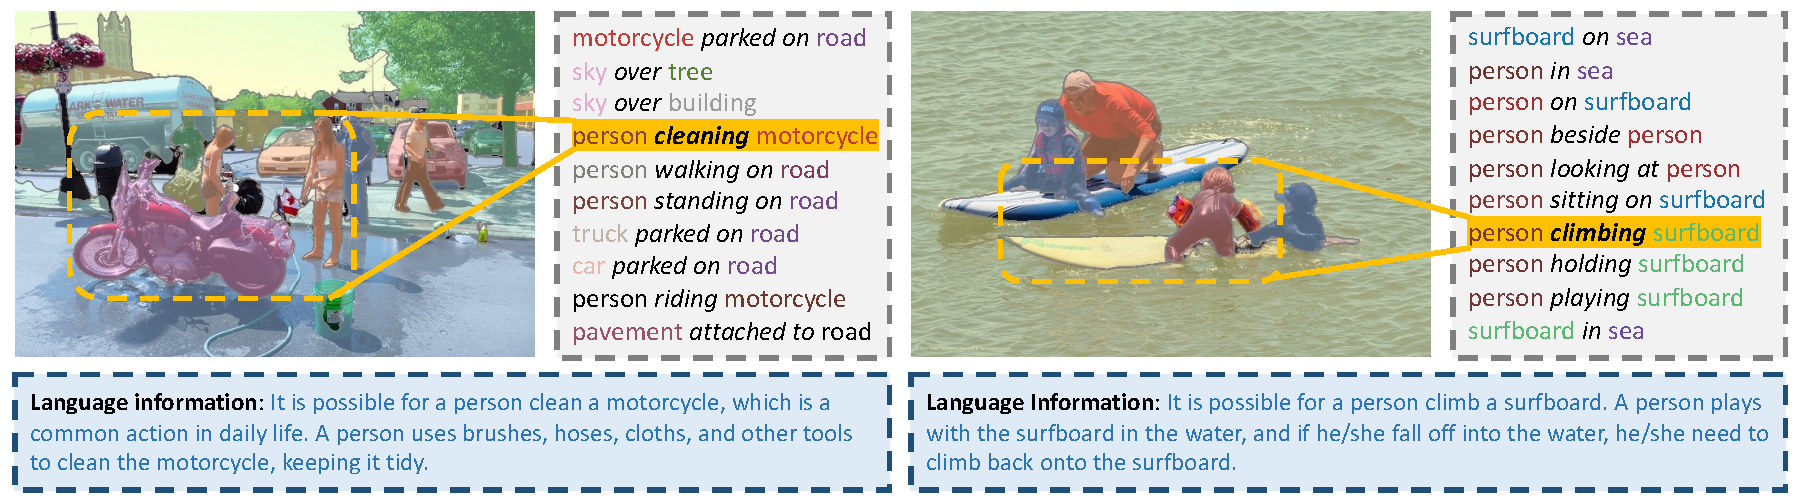
\includegraphics[width=1.0\linewidth]{Chapter4/Figures/vis_v1.pdf}
    \vspace{-4mm}
    \caption{Visualization results of our VLPrompt.
    We show two examples.
    For each example, the top left displays the predicted segmentation results, the top right shows the top 10 predicted relation triplets (all are correct relation triplets), and bottom is the language snippet utilized for predicting the highlighted triplets in yellow.
    }
    \vspace{-4mm}
    \label{vlprompt:fig:vis}
\end{figure}



\noindent \textbf{Failure case analysis.}
In addition to the high-quality visual results shown above, we also conduct a detailed failure case analysis, as illustrated in Fig.~\ref{vlprompt:fig:failure_vis}.
We observe that when multiple objects of the same category appear in close proximity within a scene, the model tends to mispredict the relations between them.
For example, in the first image from the left, 0\_person is only \textit{wearing} 3\_baseball\_glove, but the model incorrectly predicts that they are also \textit{wearing} 2\_baseball\_glove.
A similar misprediction occurs for 1\_person.
In the second image, only 0\_person is actually \textit{flying} the kite, while 1\_person and 2\_person are merely \textit{looking at} it.
When similar objects are located too close together, the segmentation model may mistakenly identify them as a single instance.
For example, in the fourth image, the model predicts that both 0\_person and 1\_person are \textit{riding} 2\_horse, whereas 2\_horse should be segmented into two separate horses instead of one.
Although incorporating language knowledge extracted from LLMs significantly alleviates the long-tail problem, reasoning about fine-grained relations between spatially adjacent objects remains a challenging issue that requires further investigation.


\noindent \textbf{Alleviating the long-tail problem.}
In SGG and PSG tasks, mR@K is often used as a reflection for a method's ability to solve long-tail problem~\citep{tang2020unbiased}.
To further validate it, in PSG dataset, we split relations occurring over 1000 times as common relations, and those under 1000 as rare relations, resulting into 21 common and 35 rare relations.
As shown in Tab.~\ref{vlprompt:tab:long_tail_psg}, our method's integration of language information (w/ LLM) leads to 2.3 increase in mR@100 for common relations and 13.8 increase for rare relations on the PSG dataset.
Tab.~\ref{vlprompt:tab:long_tail_vg} reveals consistent findings on the VG dataset.
The significant improvement in the latter highlights the effectiveness in enhancing rare relation prediction.
Additionally, as shown in Fig.~\ref{vlprompt:fig:predicate_wise}, we present relation/predicate-wise performance improvements on PSG dataset, further highlighting the effectiveness of our method across different relations.
Note, w/o LLM is our method without language information (Sec.~\ref{vlprompt:sec:method}).
In this setting, we remove the cross-attention module and rely solely on vision features for relation prediction.

\begin{table}[!t]
    \centering
    \setlength{\tabcolsep}{2.0mm}
    \caption{Alleviating the long-tail problem on PSG dataset.
    Incorporating LLM-based language information boosts performance on common and rare relations, with greater gains for rare ones, validating its effectiveness in addressing the long-tail problem.}
    % \resizebox{1.0\linewidth}{!}{
    \begin{tabular}{l|cccc}
    \toprule[1.3pt]
    ~ & \multicolumn{2}{c}{Common relations} & \multicolumn{2}{c}{Rare relations}\\
    ~ & w/o LLM & w/ LLM & w/o LLM & w/ LLM\\
    \midrule
    mR@100 & 54.7 & \textbf{57.0 (\textcolor{darkgreen}{+2.3})} & 37.9 & \textbf{51.7 (\textcolor{darkgreen}{+13.8})} \\
    \bottomrule[1.3pt]
    \end{tabular}
    % }
    \label{vlprompt:tab:long_tail_psg}
\end{table}


\begin{table}[!t]
    \centering
    \setlength{\tabcolsep}{2.0mm}
    \caption{Alleviating the long-tail problem on VG dataset.}
    % \resizebox{1.0\linewidth}{!}{
    \begin{tabular}{l|cccc}
    \toprule[1.3pt]
    ~ & \multicolumn{2}{c}{Common relations} & \multicolumn{2}{c}{Rare relations}\\
    ~ & w/o LLM & w/ LLM & w/o LLM & w/ LLM\\
    \midrule
    mR@100 & 21.6 & \textbf{23.2 (\textcolor{darkgreen}{+1.6})} & 9.7 & \textbf{16.4 (\textcolor{darkgreen}{+6.7})} \\
    \bottomrule[1.3pt]
    \end{tabular}
    % }
    \label{vlprompt:tab:long_tail_vg}
\end{table}



\begin{figure}[H]
    \centering
    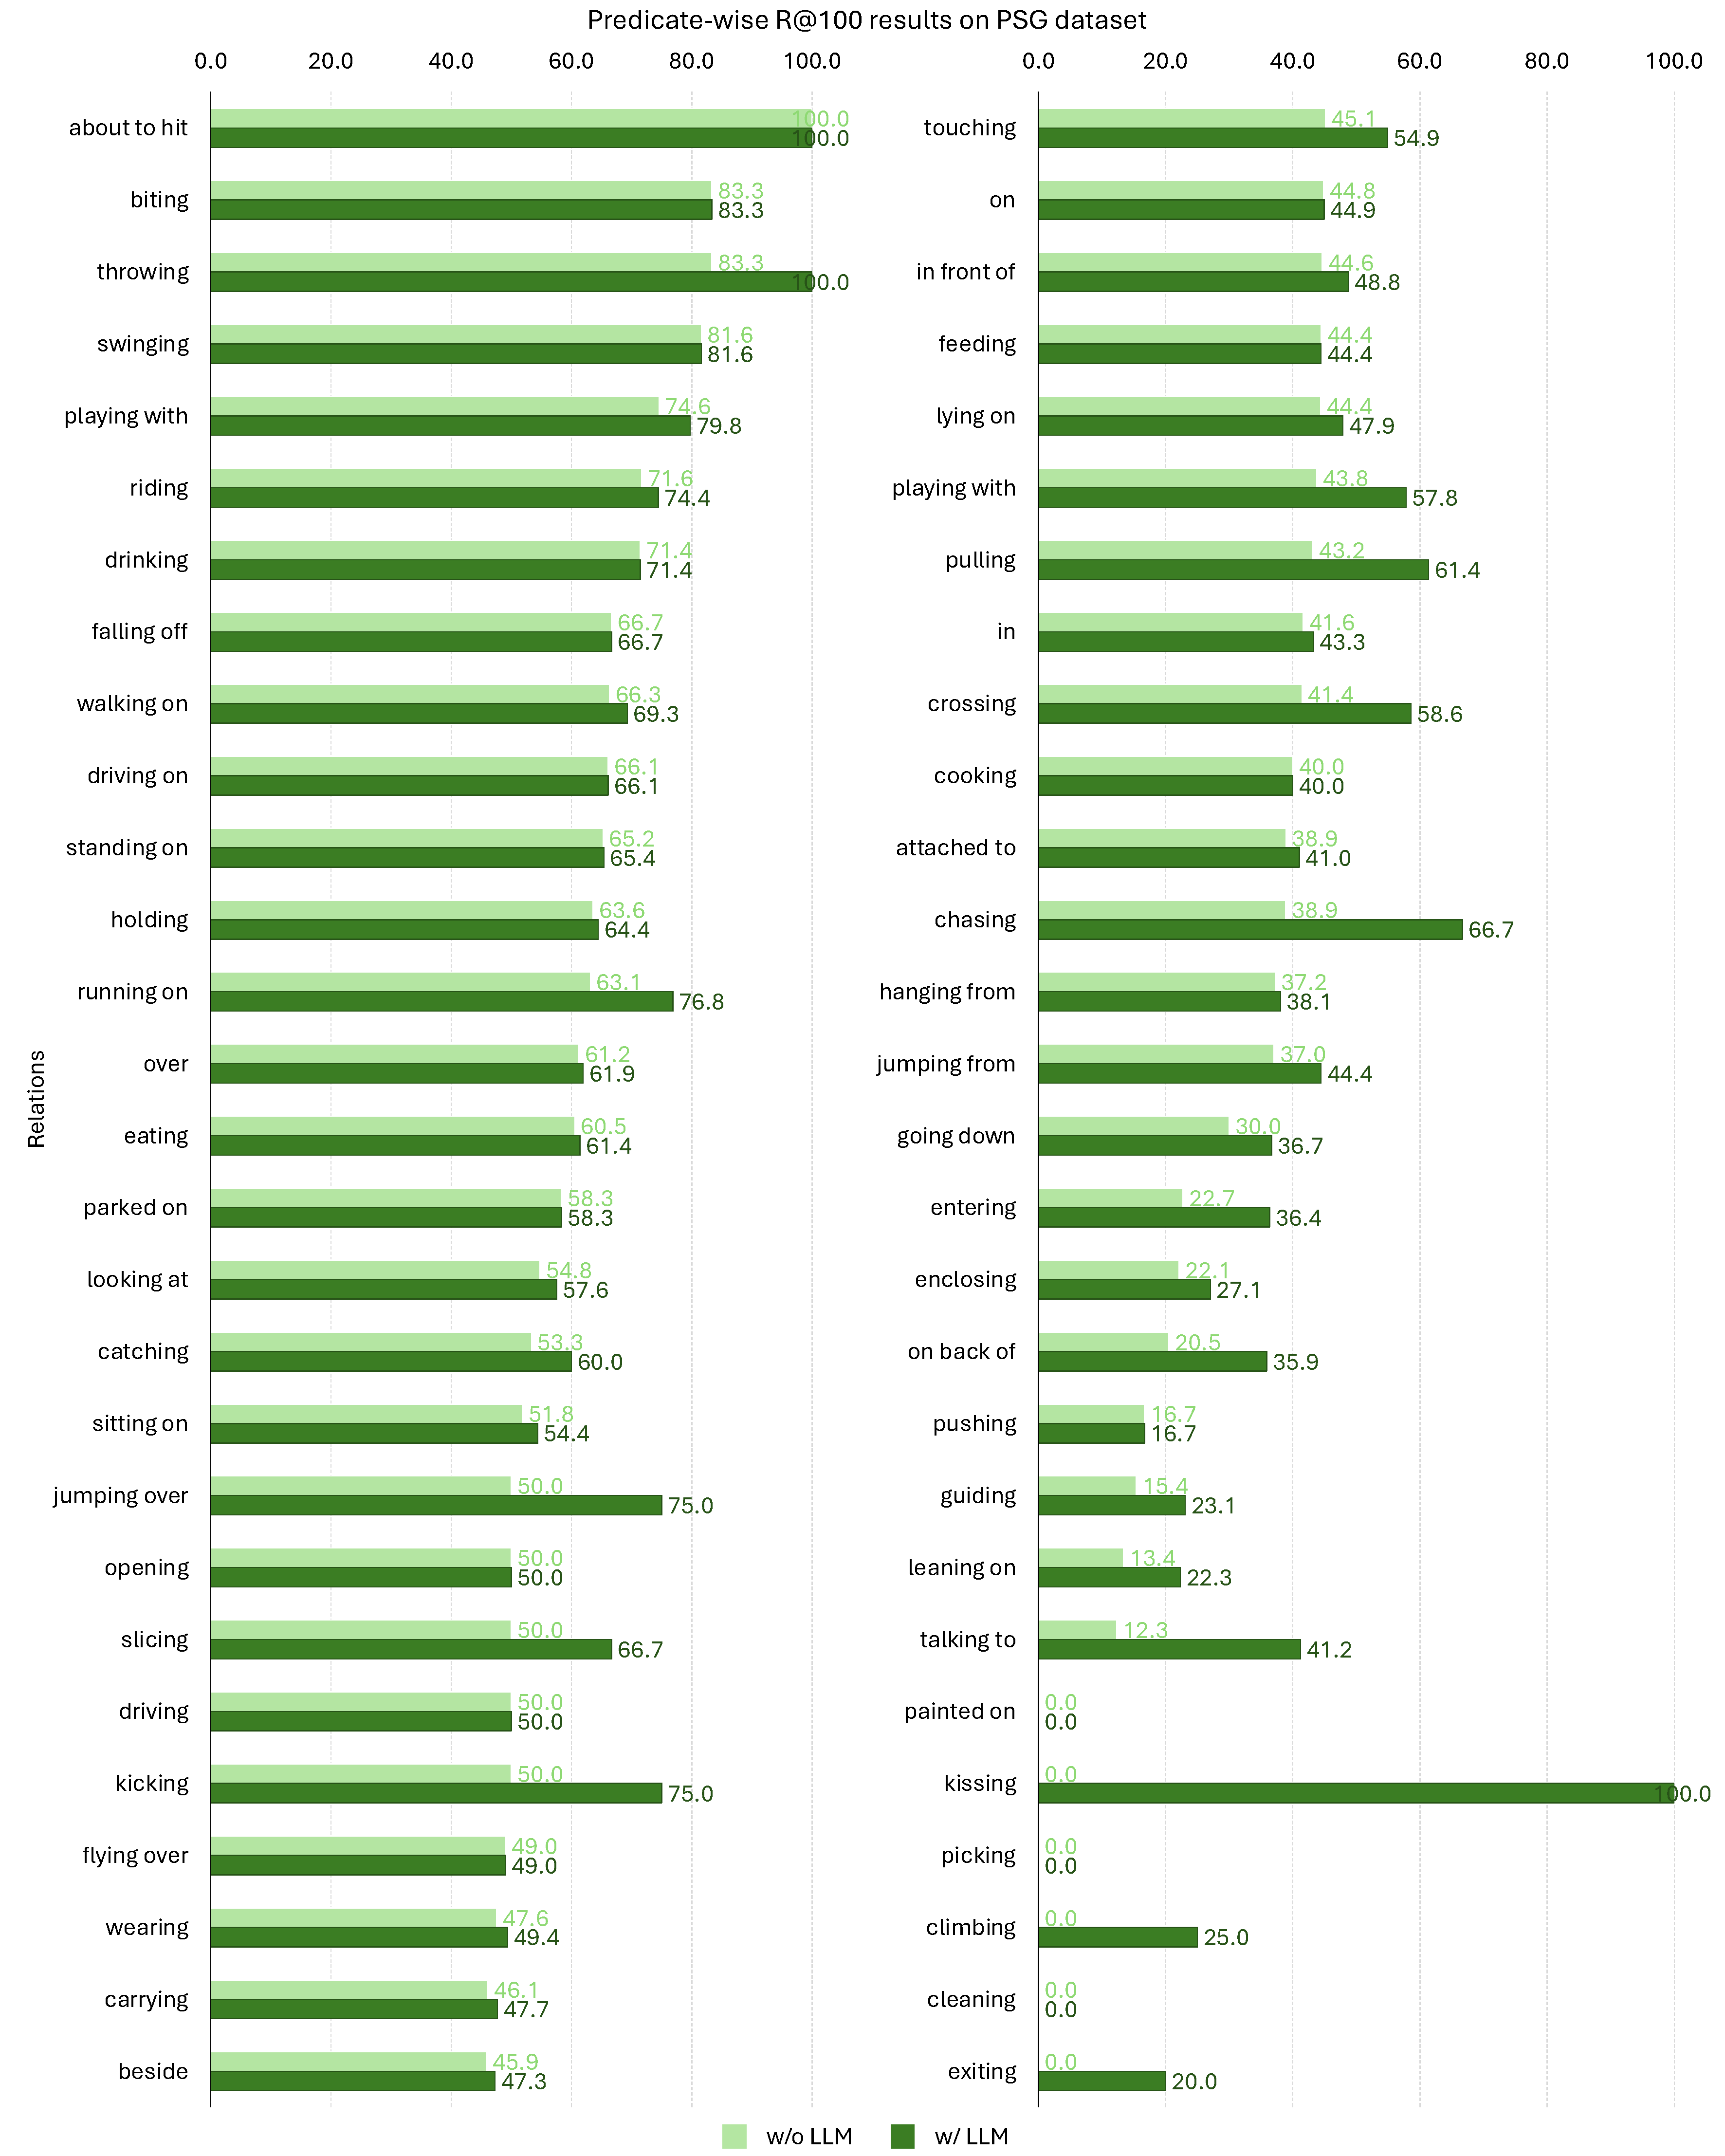
\includegraphics[width=1.05\linewidth]{Chapter4/Figures/predicate_wise_v2.pdf}
    \vspace{-2mm}
    \caption{Predicate-wise R@100 results on the PSG dataset show performance improvements across various relations with LLM integration.}
    \label{vlprompt:fig:predicate_wise}
\end{figure}



\begin{figure}[!t]
    \centering
    \begin{subfigure}{0.5\textwidth}
        \centering
        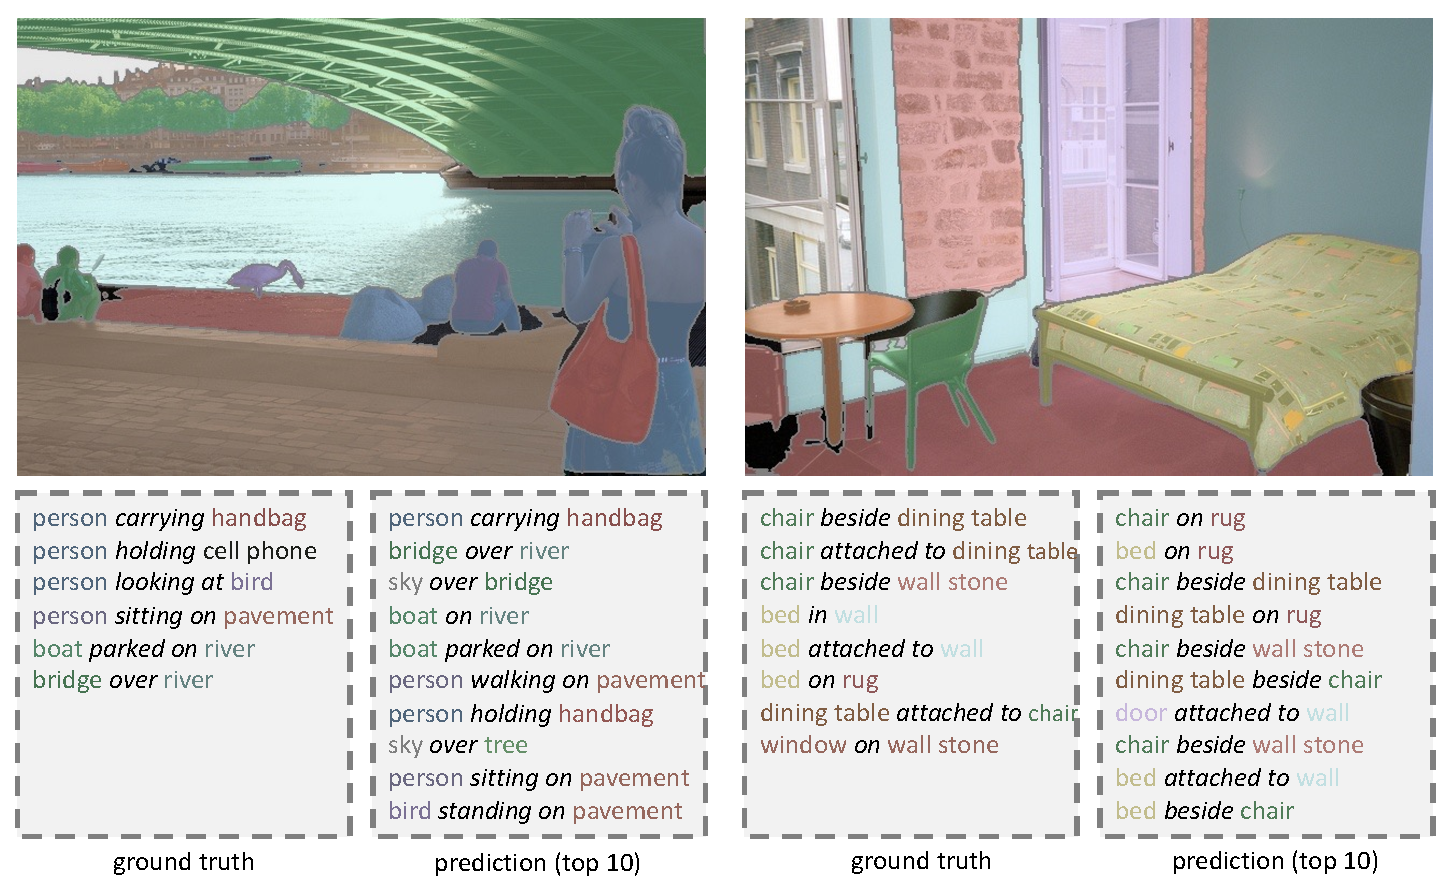
\includegraphics[width=\linewidth]{Chapter4/Figures/vis_v3.pdf}
    \end{subfigure}
    \hspace{-2mm}
    \begin{subfigure}{0.5\textwidth}
        \centering
        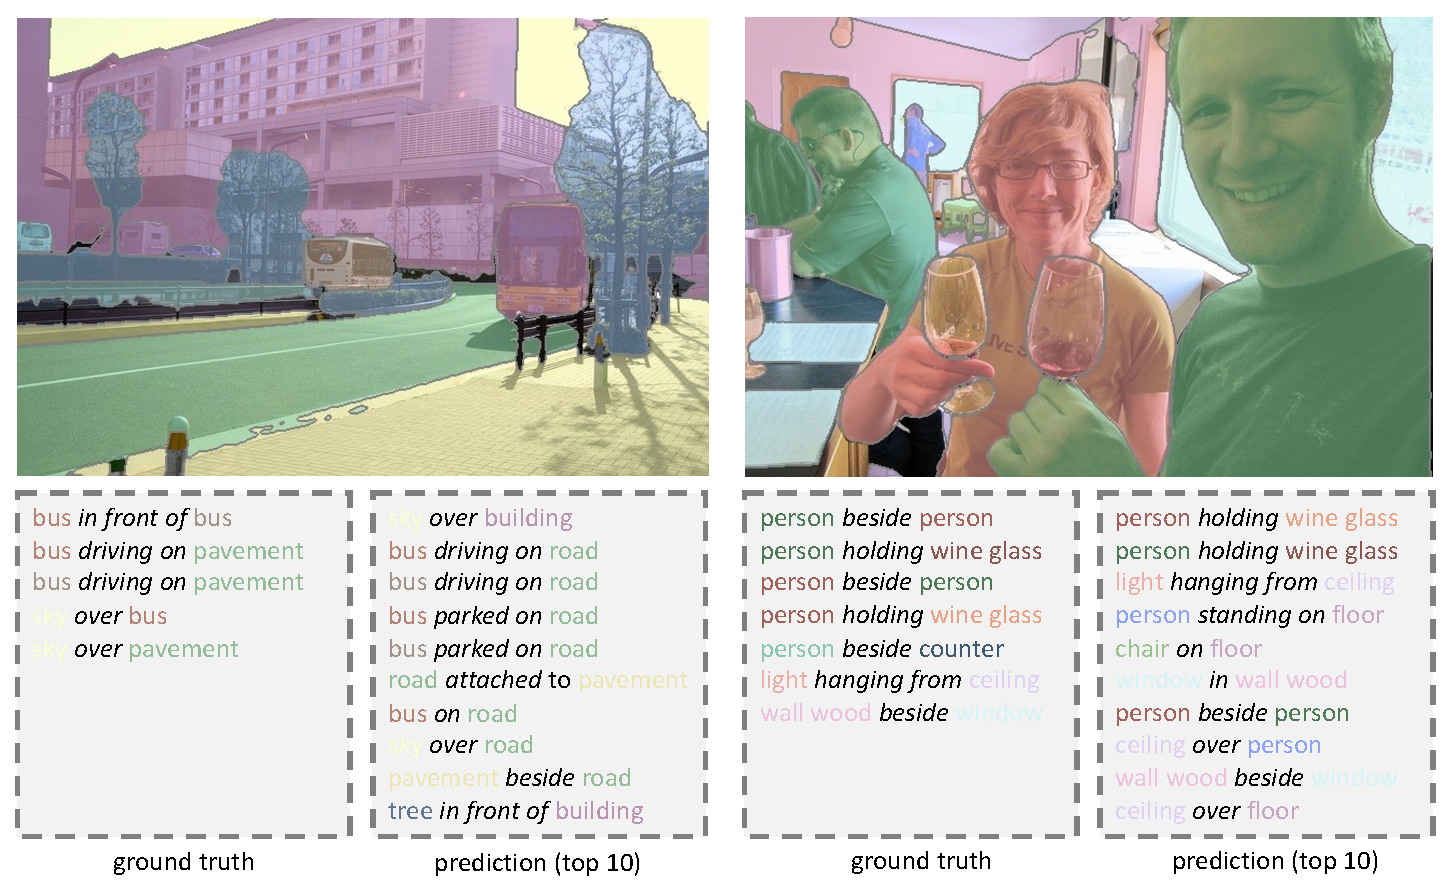
\includegraphics[width=\linewidth]{Chapter4/Figures/vis_v4.pdf}
    \end{subfigure}
    \begin{subfigure}{0.5\textwidth}
        \centering
        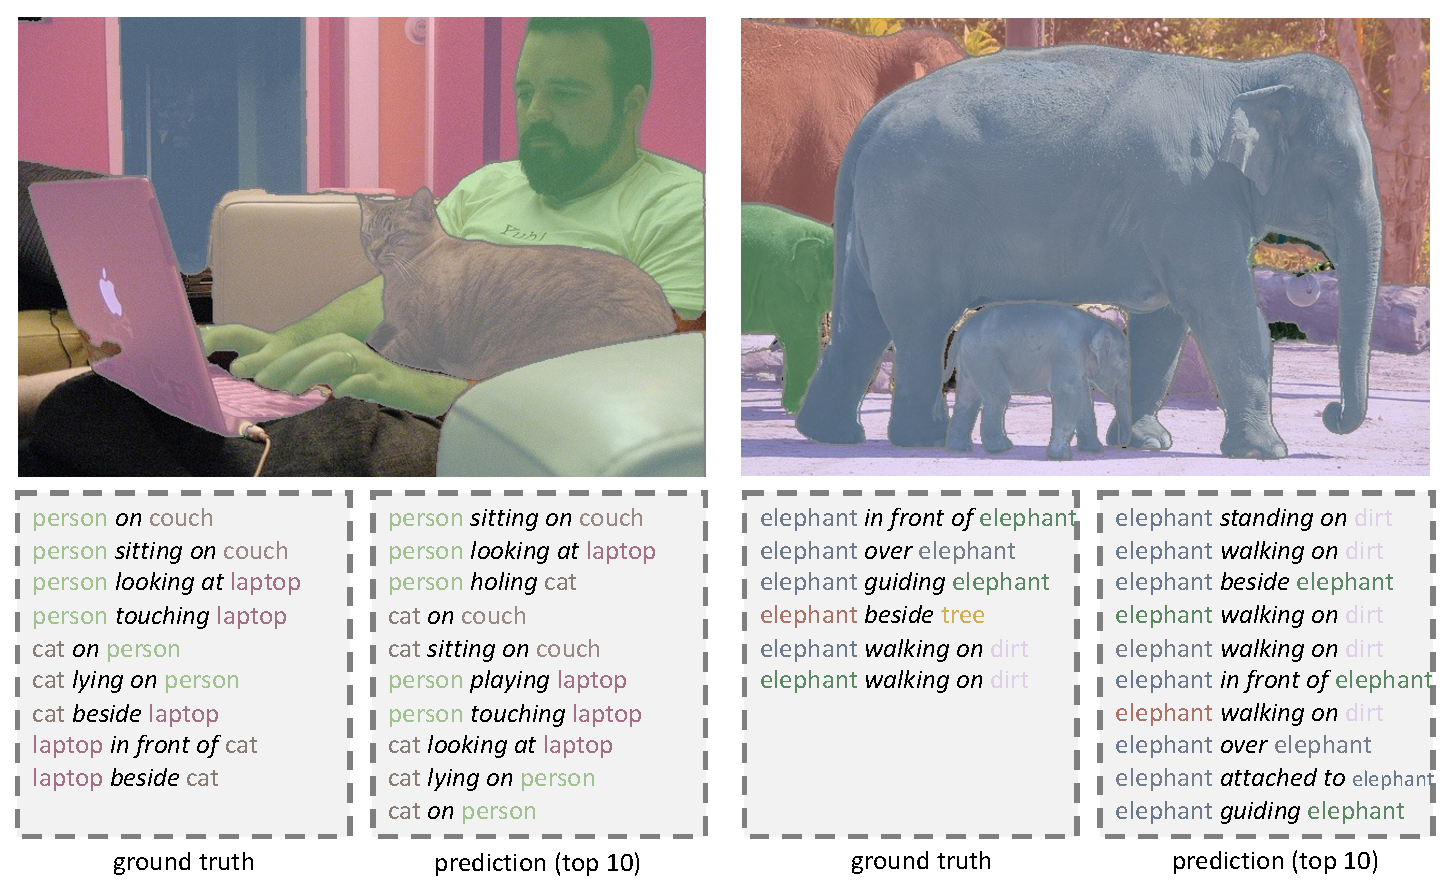
\includegraphics[width=\linewidth]{Chapter4/Figures/vis_v6.pdf}
    \end{subfigure}
    \hspace{-2mm}
    \begin{subfigure}{0.5\textwidth}
        \centering
        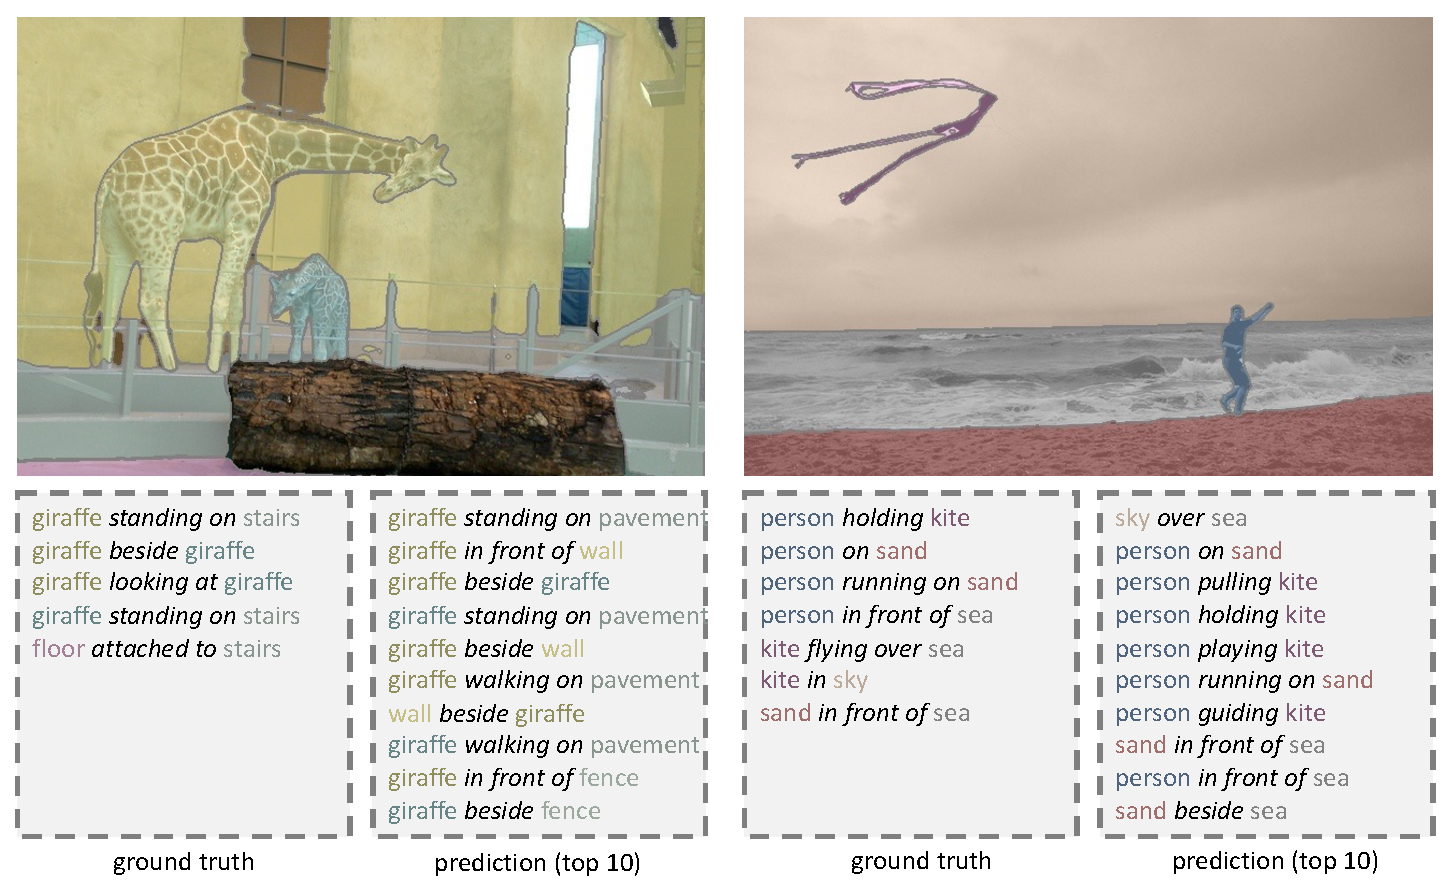
\includegraphics[width=\linewidth]{Chapter4/Figures/vis_v7.pdf}
    \end{subfigure}
    \caption{Visualization of panoptic segmentation (top), ground truth (bottom left), and top 10 relation predictions (bottom right) demonstrates VLPrompt's precision in relation prediction, enhancing scene understanding.}
    \label{vlprompt:fig:more_vis}
    \vspace{-6mm}
\end{figure}



\begin{figure}[!t]
    \centering
    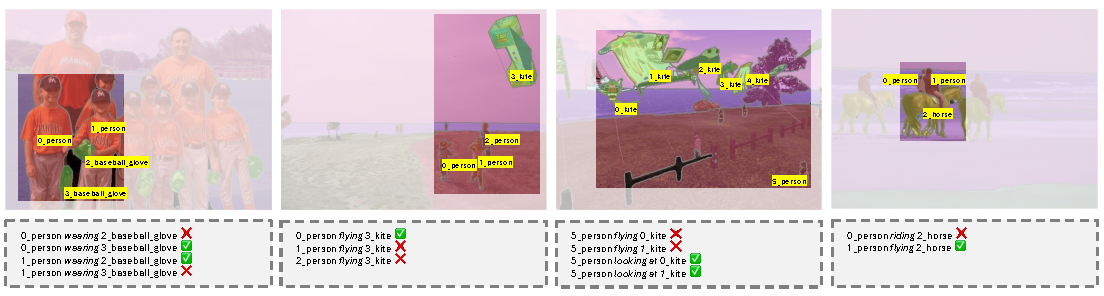
\includegraphics[width=1.0\linewidth]{Chapter4/Figures/failure_case_analysis_v2.pdf}
    \vspace{-4mm}
    \caption{Visualization of typical failure cases.
    We visualize typical failure cases of VLPrompt, which mainly occur when multiple instances of the same object category appear in the scene.
    In such cases, the model often mismatches the relations between different objects.
    }
    \vspace{-4mm}
    \label{vlprompt:fig:failure_vis}
\end{figure}



\noindent \textbf{Comparison with large multimodal models.}
Large multimodal models (LMMs) currently demonstrate great performance across various multimodal tasks and can also predict relations with specific instructions.
To further validate the performance of LMMs on PSG task, we test three popular LMMs GPT-4o, GPT-4V and Llama 3.2-11B on the PSG test set.
To ensure fairness in comparison, we allow LMMs to use the segmentation results output by our method, thus ensuring same segmentation performance.
Specifically, following the approach of \citet{yang2023setofmark}, we attach the panoptic segmentation results extracted by our model to the original image and input it to LMMs.
This allows LMMs to obtain object segmentation results and the corresponding categories consistent with our method.
Subsequently, we use LMMs to predict the relations for all object pairs.
From the experimental results, as shown in Tab.~\ref{vlprompt:tab:gpt_4v}, we observe that as more advanced LMMs are used, their performance steadily improves.
However, a noticeable performance gap still remains compared to our PSG model.
This trend indicates that LMMs hold strong potential for achieving better results.
In turn, we believe that future advances in LMMs may further promote progress in panoptic scene graph generation.

\begin{table}[!t]
    \centering
    \setlength{\tabcolsep}{1.2mm}
    \caption{Comparison with LMMs in PSG task.
    Large multimodal models like GPT-4V, not tailored for PSG task, underperform compared to task-specific PSG models.}
    % \resizebox{1.0\linewidth}{!}{
    \begin{tabular}{l|cccccc}
    \toprule[1.3pt]
    Method & R@20 & mR@20 & R@50 & mR@50 & R@100 & mR@100 \\
    \midrule
    VLPrompt & \textbf{39.4} & \textbf{34.7} & \textbf{47.6} & \textbf{45.1} & \textbf{52.4} & \textbf{53.7} \\
    GPT-4o~\citep{chatgpt} & 30.9 & 28.6 & 40.2 & 38.9 & 45.9 & 44.1 \\
    GPT-4V~\citep{chatgpt} & 16.9 & 10.1 & 20.4 & 12.8 & 22.5 & 13.1 \\
    Llama 3.2-11B~\citep{dubey2024llama} & 14.8 & 6.9 & 16.9 & 8.2 & 18.1 & 9.5 \\
    \bottomrule[1.3pt]
    \end{tabular}
    % }
    \label{vlprompt:tab:gpt_4v}
\end{table}


\subsection{Ablation study}

\subsubsection{Vision Feature Extractor}

\begin{table}[!t]
    \centering
    \setlength{\tabcolsep}{1.2mm}
    \caption{Ablation study for the Vision Feature Extractor.}
    % \resizebox{1.0\linewidth}{!}{
    \begin{tabular}{l|cccccc}
    \toprule[1.3pt]
    Method & R@20 & mR@20 & R@50 & mR@50 & R@100 & mR@100 \\
    \midrule
    VLPrompt & \textbf{39.4} & \textbf{34.7} & \textbf{47.6} & \textbf{45.1} & \textbf{52.4} & \textbf{53.7} \\
    ~~~~PixelDec $\rightarrow$ TsfmDec & 37.4 & 32.1 & 45.8 & 43.7 & 50.1 & 50.3 \\
    ~~~~MaskPool $\rightarrow$ BboxPool & 38.6 & 33.7 & 46.4 & 44.8 & 51.0 & 52.6 \\
    ~~~~Concat. $\rightarrow$ Sub. & 35.4 & 29.8 & 44.1 & 42.3 & 48.6 & 48.9 \\
    ~~~~w/o Spatial Feat. & 39.0 & 33.0 & 46.6 & 44.3 & 51.7 & 52.1 \\
    \bottomrule[1.3pt]
    \end{tabular}
    % }
    \label{vlprompt:tab:ablation_vision_feature_extractor}
\end{table}

\noindent \textbf{Object features from pixel decoder.}
To validate the superiority of obtaining object features from the pixel decoder (PixelDec) of Mask2Former, we experiment with an alternative approach: acquiring corresponding object features from the transformer decoder (TsfmDec) of Mask2Former. This is a common practice in the literature~\citep{cong2023reltr}.
Experiments (PixelDec$\rightarrow$TsfmDec) in Tab.~\ref{vlprompt:tab:ablation_vision_feature_extractor} show that the feature from the pixel decoder performs 3.4 better in mR@100 than that from the transformer decoder, as the pixel decoder contains more comprehensive vision information.

\noindent \textbf{Mask pooling for object feature extraction.}
Common methods to obtain object features from the pixel decoder include mask pooling (MaskPool) and bounding box pooling (BboxPool)~\citep{girshick2015fast}.
We validate our choice of mask pooling through ablation experiments (MaskPool$\rightarrow$BboxPool).
As shown in Tab.~\ref{vlprompt:tab:ablation_vision_feature_extractor}, the performance using mask pooling is 1.1 higher in mR@100 than that using bbox pooling.
Mask pooling is more suitable for the mask prediction in the PSG task. 

\noindent \textbf{Concatenating object features into a pair feature.}
Common methods for merging the features of two objects for their relation prediction include concatenation (Concat.) \citep{zhang2019graphical} and subtraction (Sub.) \citep{cheng2022visual}.
Notably, addition of the features cannot be used due to the inherent order requested between the subject and object.
Results (Concat.$\rightarrow$Sub.) in Tab.~\ref{vlprompt:tab:ablation_vision_feature_extractor} indicate that concatenation outperforms subtraction by 4.8 on the mR@100.

\noindent \textbf{Spatial feature.}
To validate the effect of adding spatial features, we conduct an ablation study by removing these features.
The results (w/o Spatial Feat.) in Tab.~\ref{vlprompt:tab:ablation_vision_feature_extractor} show that this leads to a decrease of -0.7 in R@100 and -1.6 in mR@100.
This is because spatial features provide the model with additional spatial interaction between the subject and object (Sec.~\ref{vlprompt:sec:vision_feature_extractor}), thereby enhancing the vision feature for relation prediction.


\subsubsection{Language Feature Extractor}

\begin{table}[!t]
    \centering
    \setlength{\tabcolsep}{1.2mm}
    \caption{Ablation study for the Language Feature Extractor.}
    % \resizebox{1.0\linewidth}{!}{
    \begin{tabular}{l|cccccc}
    \toprule[1.3pt]
    Method & R@20 & mR@20 & R@50 & mR@50 & R@100 & mR@100 \\
    \midrule
    VLPrompt & \textbf{39.4} & \textbf{34.7} & \textbf{47.6} & \textbf{45.1} & \textbf{52.4} & \textbf{53.7} \\
    ~~~~w/o CoT & 36.8 & 27.9 & 44.3 & 38.8 & 48.6 & 45.7 \\
    ~~~~w/o template & 39.0 & 33.7 & 47.0 & 43.8 & 51.6 & 52.2 \\
    ~~~~Ext$^\text{RP} \rightarrow$ Ext$^\text{RJ}$ & 39.1 & 34.2 & 47.5 & 45.1 & 52.3 & 53.5 \\
    ~~~~Ext$^\text{RJ} \rightarrow$ Ext$^\text{RP}$ & 38.9 & 31.2 & 46.8 & 41.7 & 51.0 & 49.9 \\
    ~~~~Swap(Ext$^\text{RP}$, Ext$^\text{RJ}$)~~~~ & 36.2 & 29.4 & 44.3 & 38.6 & 48.7 & 46.4 \\
    ~~~~Llama3-8B + Bert & 39.0 & 33.5 & 47.3 & 44.8 & 52.0 & 53.2 \\
    ~~~~Compression & 38.3 & 33.1 & 46.5 & 44.6 & 51.2 & 51.1 \\
    \bottomrule[1.3pt]
    \end{tabular}
    % }
    \label{vlprompt:tab:ablation_language_feature_extractor}
\end{table}

\noindent \textbf{Chain-of-thought for prompt.}
By carefully designing prompts with the chain-of-thought technique, LLMs can produce rich and accurate descriptions.
However, if we do not use chain-of-thought and instead directly ask LLMs questions, such as replacing the relation proposer prompt with ``What are the possible relations between subject and object? And why?'' or the relation judger prompt with ``Could this relation be possible between subject and object? Why?", we find that the outputs from LLMs become much less predictable and often not as expected.
We experiment without chain-of-thought (w/o CoT) and the results in Tab.~\ref{vlprompt:tab:ablation_language_feature_extractor} show that the performance of relation prediction significantly drops, \ie, a -8.0 decrease in mR@100.
This further illustrates the rationale and importance of using chain-of-thought technology for designing prompts.

\noindent \textbf{Template phrase in RP-prompt.}
The template phrase appended to the end of the RP-prompt helps the model clearly distinguish common relations from less plausible ones, thereby preventing performance degradation on high-frequency relations during prediction.
To validate this design, we conduct an ablation study by removing the template phrase.
As shown in Tab.~\ref{vlprompt:tab:ablation_language_feature_extractor} (w/o template), excluding the template leads to a slight performance drop ($-0.8$ R@100, $-1.5$ mR@100), indicating that explicitly guiding the model to differentiate between common and uncommon relations through prompt design is beneficial.

\noindent \textbf{Different feature extraction methods.}
To validate our design of different feature extract methods for RP- and RJ-language prompting features, we study their effects.
We offer three variants:
1) For RP-language prompting features, we adopt the same way as the RJ-language prompting feature to extract feature for each relation triplet individually, we denote this variant as Ext$^\text{RP} \rightarrow$ Ext$^\text{RJ}$ in the Tab.~\ref{vlprompt:tab:ablation_language_feature_extractor}.
It shows that performance is slightly lower than our original VLPrompt, but with increased computation.
2) For RJ-language prompting features, we adopt the same way as the RP-language prompting feature to extract all relation triplets into one feature, denoted by Ext$^\text{RJ} \rightarrow$ Ext$^\text{RP}$ in the Tab.~\ref{vlprompt:tab:ablation_language_feature_extractor}.
We observe a clear drop in mR@K, as this would condense the features of relations between subject and object while dropping the subtle details, which can be especially disadvantageous for rare relations.
3) We swap the feature extraction methods between Ext$^\text{RP}$ and Ext$^\text{RJ}$, denoted by Swap(Ext$^\text{RP}$, Ext$^\text{RJ}$) in Tab.~\ref{vlprompt:tab:ablation_language_feature_extractor}.
We observe a substantial decrease in both metrics.
Our original feature extraction is specifically designed on one side to focus on the condensed and distinct attributes of commonly occurring relations; on the other side to focus on the detailed and subtle attributes of all possible especially rare relations for a subject-object pair.

\noindent \textbf{Different LLMs and text encoders.}
To further assess the effects of different LLMs and text encoders on model performance, we attempt to replace the GPT-4 with Llama3-8B~\citep{touvron2023llama} and the OpenAI Embedding Service with Bert~\citep{devlin2018bert}.
When using Bert, we take the mean of the embeddings of all output tokens as the feature.
The experimental results (Llama3-8B + Bert) in Tab.~\ref{vlprompt:tab:ablation_language_feature_extractor} reveal that using Llama3-8B as the LLM and Bert as the text encoder results in only a slight decrease in performance: -0.4 in R@100 and -0.5 in mR@100.
We review the descriptions output by Llama3-8B and compare them with those from GPT-4, finding no significant differences in quality, more details can be found in supplementary materials.
This suggests that, with carefully designed prompts, open-source LLMs with reduced parameters also work for our method, thus validating the flexibility of our method.

\noindent \textbf{Compress the language prompting feature.}
At runtime, the language prompting feature occupies 290.57MB of memory, which is manageable.
To further enhance the model's applicability in real-world scenarios, such as when there are more object and relation categories, we compress the language prompting feature to 1/4 of its original size using an encoder-decoder models.
Results (Compression) shown in Tab.~\ref{vlprompt:tab:ablation_language_feature_extractor} indicate that compressing the language prompting feature to 1/4 leads to only a minor performance decrease, while the memory required by the model during runtime is reduced to 1/4 of the original, which further demonstrates the practicality of our method in real-world settings.



\subsubsection{Vision-Language Prompter}

\begin{table}[!t]
    \centering
    \setlength{\tabcolsep}{1.2mm}
    \caption{Ablation study for the Vision-Language Prompter.}
    % \resizebox{1.0\linewidth}{!}{
    \begin{tabular}{l|cccccc}
    \toprule[1.3pt]
    Method & R@20 & mR@20 & R@50 & mR@50 & R@100 & mR@100 \\
    \midrule
    VLPrompt & \textbf{39.4} & \textbf{34.7} & \textbf{47.6} & \textbf{45.1} & \textbf{52.4} & \textbf{53.7} \\
    ~~~~w/o Language~~~~~~ & 37.1 & 26.8 & 45.9 & 37.2 & 50.0 & 44.2 \\
    ~~~~RP-decoder & 38.4 & 30.6 & 46.6 & 41.2 & 50.9 & 49.6 \\
    ~~~~RJ-decoder & 37.9 & 34.2 & 45.3 & 44.6 & 50.4 & 52.8 \\
    ~~~~Uncompressed $F_L^{RJ}$ for $W^{RJ}$ & 39.3 & 34.7 & 47.5 & 44.9 & 52.1 & 53.7 \\
    \bottomrule[1.3pt]
    \end{tabular}
    % }
    \label{vlprompt:tab:ablation_vision_language_prompter}
    \vspace{-2mm}
\end{table}

\noindent \textbf{Language information.}
To validate the efficacy of incorporating language information, we conduct a comparative experiment by replacing all language prompting features in the vision-language prompter with vision prompting features.
This approach ensures that all other factors remain constant while assessing the impact of language information.
As shown in Tab.~\ref{vlprompt:tab:ablation_vision_language_prompter}, the experimental results (w/o Language) reveal a significant decrease in the mR@100 by -9.5 when language information is removed, which demonstrates the substantial impact of language information in mitigating the long-tail problem.

\noindent \textbf{Results of RP-decoder and RJ-decoder.}
We test the relation prediction performance of both RP-decoder and RJ-decoder separately.
The results (RP-decoder and RJ-decoder) in Tab.~\ref{vlprompt:tab:ablation_vision_language_prompter} show that the RP-decoder outperforms the RJ-decoder in the R@K (\eg, 50.9 \vs 50.4 for R@100), while the RP-decoder scores lower in mR@K compared to the RJ-decoder (\eg, 49.6 \vs 52.8 for mR@100).
This indicates that the RP-decoder is good at predicting frequent relation classes, whereas the RJ-decoder excels in rare relation classes, which indicates that they are complementary.

\noindent \textbf{Relation fusion.}
As shown in Tab.~\ref{vlprompt:tab:ablation_vision_language_prompter}, when the outputs of the two branches are combined via our relation fusion strategy (\ie, VLPrompt), the final prediction outperforms either individual branch, demonstrating the effectiveness of our design.
Specifically, the RP-decoder achieves higher R@K but lower mR@K scores compared to the RJ-decoder, as it receives RP-language prompting features that encode the most frequent relations for each subject-object pair.
This makes the model more biased toward high-frequency relations, resulting in strong performance on common categories but poor generalization to rare ones, due to the long-tail distribution of relation labels.
In contrast, the RJ-decoder, which uses RJ-language prompting features to independently judge each relation category, achieves better mR@K at the cost of slightly reduced R@K, as it improves rare-relation prediction by sacrificing some performance on frequent ones.
These complementary behaviors highlight the importance of integrating both decoders, allowing the model to leverage their respective strengths and achieve overall optimal performance.

\noindent \textbf{Fusion weights.}
The input feature $F_L^{RJ}$ used to compute the fusion weights $W^{RJ}$ is compressed along the relation dimension, and this operation is applied solely within the gate network.
Our empirical results show that this compression has minimal impact on performance, as the gate network is only responsible for generating fusion weights.
To validate this design choice, we conduct an ablation study.
As shown in Tab.~\ref{vlprompt:tab:ablation_vision_language_prompter} (Uncompressed $F_L^{RJ}$ for $W^{RJ}$), using the uncompressed $F_L^{RJ}$ yields performance comparable to its compressed counterpart.
This confirms that the compressed version of $F_L^{RJ}$ offers a more computationally efficient implementation without sacrificing performance.



\begin{table}[!t]
    \centering
    \setlength{\tabcolsep}{1.2mm}
    \caption{Ablation study for the number of decoder blocks.}
    % \resizebox{1.0\linewidth}{!}{
    \begin{tabular}{c|cccccc}
    \toprule[1.3pt]
    ~~~~~Block Number~~~~~ & R@20 & mR@20 & R@50 & mR@50 & R@100 & mR@100 \\
    \midrule
    1 & 35.1 & 29.8 & 44.8 & 39.5 & 47.2 & 46.9 \\
    2 & \textbf{39.4} & 34.7 & \textbf{47.6} & 45.1 & \textbf{52.4} & 53.7 \\
    4 & 38.9 & \textbf{34.8} & 47.4 & \textbf{45.2} & 52.1 & \textbf{53.9} \\
    12 & 18.4 & 14.5 & 27.5 & 23.0 & 33.2 & 29.4 \\
    \bottomrule[1.3pt]
    \end{tabular}
    % }
    \label{vlprompt:tab:ablation_decoder_block_number}
\end{table}

\noindent \textbf{The number of decoder blocks.}
To elucidate the reason that both RP-decoder and RJ-decoder use a 2-block transformer decoder, we vary different numbers of blocks in Tab.~\ref{vlprompt:tab:ablation_decoder_block_number}.
We observe that when increasing the transformer decoder blocks from 1 to 2, there is a significant improvement in model performance.
However, increasing from 2 to 4 blocks does not change much for the performance.
Further increasing the decoder blocks to 12 leads to a notable decrease in performance, suggesting that too many decoder blocks may cause the model to overfit.
Considering both performance and speed, we choose 2 blocks.


\subsubsection{Efficiency Analysis}

\begin{table}[!t]
    \centering
    \caption{Analysis for efficiency.
    Our method achieves significant performance improvements without introducing notable efficiency issues, maintaining a comparable level to previous approaches.
    }
    % \resizebox{0.8\linewidth}{!}{
    \begin{tabular}{l|ccc}
    \toprule[1.3pt]
    Method & FLOPS (G) & Parameters (G) & Inference Speed (ms) \\
    \midrule
    PSGTR \citep{yang2022panoptic} & 461.3 & 44.2 & 140 \\
    HiLo \citep{zhou2023hilo} & 229.4 & 58.7 & 156 \\
    VLPrompt (ours) & 386.7 & 49.1 & 152 \\
    \bottomrule[1.3pt]
    \end{tabular}
    % }
    \label{vlprompt:tab:analysis_efficiency}
\end{table}

In Tab.~\ref{vlprompt:tab:analysis_efficiency}, we compare our model's efficiency with the previous state-of-the-art models, evaluating computational floating point operations per second (FLOPS), parameter size and inference speed on the same A100 GPU.
We observe that although our method has higher FLOPS compared to HiLo, it matches HiLo in prediction speed, and significantly outperforms HiLo in performance (see Tab.~\ref{vlprompt:tab:psg_results}).


\section{Limitations and Critical Reflection}
\label{sec:limitation}
Our method achieves large performance improvements on the PSG task, but several limitations and unexamined assumptions remain.

\noindent \textbf{The language information is static and pre-extracted.}
Our approach requires pre-extracting language information from LLMs before relation prediction. The extraction is efficient and cost-effective, but it creates a dependency on external models and on a preprocessing stage, which may limit scalability in some deployment settings. A more important consequence is that we elicit descriptions \emph{per category pair} rather than per image, so the descriptions are fixed at training time. This is what makes the method affordable, since the LLM is queried once for each subject-object category combination instead of once per test image. It also means that the language signal is a class-level prior rather than an instance-level observation. The model receives the same description of a person \textit{cleaning} an elephant regardless of the particular elephant in the image. When a specific instance differs from the typical case, the language branch cannot detect the difference, and the gating network can only discount the branch rather than correct it.

\noindent \textbf{Hallucination and the direction of the error.}
LLM-generated descriptions are not grounded in the image, and no component of our pipeline verifies them. An LLM asked how a person and a surfboard might be related produces fluent and plausible text whether or not that relation is present, and it describes the \emph{stereotypical} interaction because that is what its training distribution supports. The hallucination risk therefore has a specific and uncomfortable shape: the errors it introduces are biased toward the common case, which is the bias this chapter aims to reduce. The gating network is our safeguard, since it learns when to trust the language signal, but it is trained on the same long-tailed data, so its calibration in the tail is learned from few examples. Our ablation shows that GPT-4 and Llama3-8B descriptions perform comparably (Sec.~\ref{vlprompt:sec:experiments}), which is reassuring about robustness to the choice of LLM. It does not show that either set of descriptions is factually grounded, because two models that share a stereotype produce equally consistent and equally unfounded text. A stronger design would score descriptions against visual evidence before fusion, instead of leaving the entire decision to a learned gate.

\noindent \textbf{The improvements are measured against an incomplete annotation.}
As discussed in Sec.~\ref{hilo:sec:limitations}, R@$K$ and mR@$K$ score predictions against PSG annotations that are known to omit valid relations. The central result of this chapter, a 13.8 point mR@100 gain on rare relations, is therefore a claim about agreement with a particular annotation rather than about correctness in general. The concern is sharper here than in Chapter~3. Language priors could in principle improve the metric by aligning the output distribution with the linguistic conventions that annotators themselves used, without improving visual grounding. The predicate-wise analysis and the w/o-LLM ablation argue against this reading, because the gains concentrate in relations that are semantically distinguishable rather than spreading uniformly. The experiments in this chapter cannot rule it out entirely.

\noindent \textbf{Failure is concentrated in one diagnosable case.}
The failure analysis in Sec.~\ref{vlprompt:sec:experiments} shows that errors cluster where several instances of one category appear close together. The model then attaches a relation to the wrong instance, or the panoptic backbone merges two instances into a single mask and makes the correct assignment impossible. This is a scope limit worth stating plainly. Language priors operate at the level of \emph{categories}, describing how a person relates to a baseball glove, so they carry no information about \emph{which} person or \emph{which} glove. The mechanism contributed by this chapter therefore cannot resolve its own most frequent failure mode, and progress on that case requires better instance-level grounding rather than better priors.

\noindent \textbf{Closed-set by construction.}
Our method targets closed-set relation prediction and does not support open-set relation prediction, which restricts its use in real-world settings where unseen relations occur. This restriction is architectural rather than incidental, since descriptions are enumerated over a fixed set of category pairs and the prompter outputs a distribution over a fixed predicate list. We significantly reduce the long-tail problem within the closed-set setting, but closing the gap to open-set generalization remains an important challenge. Chapter~5 addresses this gap directly by extending PSG from closed-set relation classification to open-set relation prediction with large multimodal models.

\section{Conclusion}
\label{sec:conclusion}

This chapter showed that language priors from LLMs can complement the closed-set visual modeling established in Chapter~3.
VLPrompt incorporates language information generated by LLMs to enhance PSG performance.
VLPrompt utilizes the chain-of-thought method in designing prompts, enabling LLMs to generate rich descriptions for relation prediction. 
Additionally, we develop a prompter network based on attention mechanisms to facilitate comprehensive interaction between vision and language information, achieving high-quality relation prediction.
Experiments demonstrate that our method significantly outperforms the current state-of-the-art on the PSG dataset and mitigates the long-tail problem for relations.
Together, Chapters~3 and~4 improve PSG under long-tail and ambiguous supervision while preserving visual grounding.
The next chapter extends this line beyond a fixed relation vocabulary by studying open-set panoptic scene graph generation.

